\documentclass[a4 paper]{article}
%\usepackage{minted}           %embedding code
\usepackage{amsmath, amsthm, amsfonts} %always use amsmath for symbols, amsthm for theorems 
\usepackage{graphicx}  % for pictures
%\usepackage{lipsum}  % for test text
\usepackage{multicol}    % for multicollumn text
\usepackage[bottom=2.5cm]{geometry}   %to set the margins to your liking
\usepackage[skip = 10pt, indent = 30pt]{parskip}      %to set the distance between paragraphs
\usepackage{tcolorbox}           %for literal color boxes
%\usepackage{witharrows}             % understandable, arrows for equations
\usepackage{tikz}                   %drawings and diagrams
\usetikzlibrary{positioning}        %tikz library for positioning (of nodes?)
\usepackage{pgfplots}               %plotting and graphs
\pgfplotsset{compat=1.18, width = 10cm}
\usepackage{hyperref}
\hypersetup{colorlinks = true, linkcolor = black, urlcolor = blue}
%\usepackage{fancyvrb}           % fancy formatting of verbatim
%\usepackage{fancyhdr, lastpage}
%\pagestyle{fancy} 
%\lhead{Relat\'orio experimento 4}
%\rhead{FisExpI}
%\cfoot{Página \thepage \ de \pageref{LastPage}}
%\usepackage[Bjornstrup]{fncychap} %Sonny, Glenn, Lenny, Conny, Rejne, Bjarne, Bjornstrup
%\usepackage{xcolor}      %color text
\usepackage{siunitx}    %for SI units
\usepackage{setspace}
\onehalfspacing
\usepackage{cleveref}
\usepackage[brazil]{babel}
\usepackage{caption}
\usepackage{subcaption}
\usepackage{pdfpages}
\usepackage{booktabs}
\usepackage{multirow}
\usepackage{textcomp}
\usepackage{amssymb}
\usepackage[document]{ragged2e}
\usepackage{bm}





%\setlength{\hoffset}{-2cm}
%\setlength{\voffset}{1.5cm}                     %control your margins however you want!
%\setlength{\marginparwidth}{2cm}
%\setlength{\oddsidemargin}{0cm}

%\newtheorem{theorem}{Theorem}[section]               %how you call it and how you display it
%\newtheorem{corollary}{Corollary}[theorem]


\newcommand{\parag}{\hspace{30pt}}
%\newcommand{\pd}[2]{\frac{\partial#1}{\partial#2}}


\begin{document}
\justifying
\begin{center}{\large Laboratório de Circuitos Elétricos - 02/2024 - Turma 05}\\
{\large \textbf{Experimento 2}}\\ 
31/10/2024
\end{center}

\vspace{500pt}
 \noindent\textbf{Grupo 6:}\\
 Yuri Shumyatsky - 231012826\\
Vinicius de Melo Moraes - 231036274


\vspace{30pt}
\newpage

\section{Introdução}
\parag O presente estudo aborda a aplicação dos métodos de análise nodal e análise de malha para resolver circuitos elétricos, técnicas essenciais para entender o comportamento de circuitos compostos por resistores, fontes de tensão e corrente. Esses métodos são amplamente empregados na Engenharia Elétrica e em áreas relacionadas para o desenvolvimento de sistemas eletrônicos.

O experimento, realizado no contexto da disciplina de Laboratório de Circuitos Elétricos, visa consolidar o conhecimento teórico sobre os princípios de Kirchhoff e as técnicas de análise de circuitos. A análise nodal utiliza a Lei das Correntes de Kirchhoff (LKC) para determinar a tensão em cada nó do circuito, enquanto a análise de malha emprega a Lei das Tensões de Kirchhoff (LKT) para calcular as correntes em cada malha.

Para verificar a precisão e as limitações de cada método, foram implementados circuitos práticos em bancada, e os dados e resultados obtidos são analisados e discutidos neste relatório.

\section{Materiais}
\begin{itemize}
\item Multímetro - Agilent 34410A
\item Fonte DC - Agilent E3631A
\item Protoboard
\item 1 resistor de 1,5k$\Omega$
\item 1 resistor de 1,2k$\Omega$
\item 1 resistor de 1k$\Omega$
\item 1 resistor de 1,8k$\Omega$
\item 1 resistor de 2,2k$\Omega$
\end{itemize}
Montados na seguinte configuração:
\begin{table}[h]
\centering
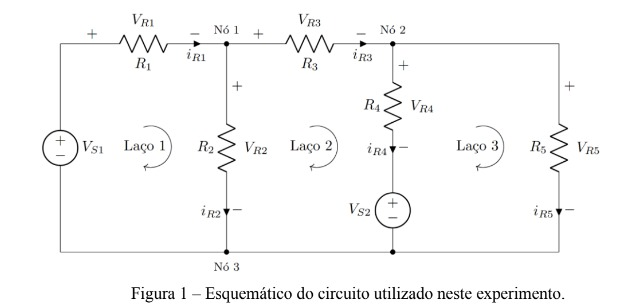
\includegraphics[scale=0.6]{figuras/figura2}
\end{table}
\\\parag Para o grupo 6, foi definido que $R_1=1k\Omega, R_2=1,2k\Omega, R_3=1,5k\Omega, R_4=1,8k\Omega$ e $R_5=2,2k\Omega, V_{S1}=2V, V_{S2}=3V$.


\newpage\section{Experimento}
\parag A primeira ação a ser tomada é verificar as resistências reais dos resistores, obtendo a Tabela 1.\\

\vspace{5pt}
\begin{table}[h]
\centering
\begin{tabular}{|c|c|c|c|}
\hline
Resistor & Valor Nominal & Valor medido & Erro (\%)\\ \hline
$R_1$ & $1k\Omega$ & $0,999k\Omega$ & 0,1  \\\hline
$R_2$ & $1,2k\Omega$ & $1,179k\Omega$ & 1,75 \\\hline
$R_3$ & $1,5k\Omega$ & $1,491k\Omega$ & 0,6 \\\hline
$R_4$ & $1,8k\Omega$ & $1,813k\Omega$ & 0,72 \\\hline
$R_5$ & $2,2k\Omega$ & $2,177k\Omega$ & 1,05 \\\hline
\end{tabular}
\caption*{Tabela 1}
\end{table}

 Em seguida serão calculadas as tensões em cada resistor e fonte, comparadas com os valores medidos experimentalmente.


Para conseguir os valores calculados das tensões, usamos as correntes encontradas com análise de malha, cujos cálculos serão expostos adiante.\\
Malha 1:\\
\[1kI_1+1,2k(I_1-I_2)=2\]
\[2,2kI_1-1,2kI_2=2\]
Malha 2:\\
\[-1,2k(I_1-I_2)+1,5kI_2+1,8k(I_2-I_3)=-3 \]
\[-1,2kI_1+4,5kI_2-1,8kI_3=-3\]
Malha 3:\\
\[-1,8k(I_2-I_3)+2,2kI_3\]

Com esse sistema, montamos a seguinte matriz:

$$
\begin{bmatrix}
2,2k & -1,2k & 0 & 2\\
-1,2k & 4,5k & -1,8k &-3\\
0 & -1,8k & 4,0k &3
\end{bmatrix}
\rightarrow
\begin{bmatrix}
1k & 3,3k & -1,8k & -1\\
0 & 1,8k & -0,84k & -0,89\\
0 & 0 & 3,16k & 2,11
\end{bmatrix}
$$

Com isso, obtemos as correntes das malhas, e usando a relação $V=RI$, calculamos as tensões em cada resistor.


\vspace{5pt}
\begin{table}[h]
\centering
\begin{tabular}{|c|c|c|c|}
\hline
Tensão & Valor calculado & Valor medido & Erro (\%)\\ \hline
$V_{R_1}$ & 0,805V  &  0,815V & 1,24\\\hline 
$V_{R_2}$ & 1,186V  &  1,180V & 0,51\\\hline
$V_{R_3}$ & -0,274V  & -0,275V & 0,36 \\\hline
$V_{R_4}$ & -1,531V  & -1,551V &1,31 \\\hline
$V_{R_5}$ & 1,469V  &  1,456V &0,88 \\\hline
$V_{S_1}$ & 2V &  1,996V & 0,20\\\hline
$V_{S_2}$ & 3V &  3,007V & 0,23\\\hline
\end{tabular}
\caption*{Tabela 2}
\end{table}


\newpage Em seguida, calcula-se as correntes em cada resistor: para $R_1, R_3, R_5$, basta usar os valores das correntes de malha calculadas no passo anterior. Para $R_2$ e $R_4$, basta fazer a soma apropriada das correntes de malha ( $R_2=I_1-I_2$ e $R_4=I_2-I_3$).

\vspace{5pt}
\begin{table}[h]
\centering
\begin{tabular}{|c|c|c|c|}
\hline
Corrente & Valor calculado & Valor medido & Erro (\%)\\ \hline
$I_{R_1} $ & 0,805mA & 0,734mA & 8,82 \\\hline 
$I_{R_2} $ & 0,988mA & 0,905mA & 8,40\\\hline
$I_{R_3} $ & -0,183mA & -0,173mA &5,46 \\\hline
$I_{R_4} $ & -0,851mA & -0,798mA &6,23 \\\hline
$I_{R_5} $ & 0,668mA & 0,630mA &5,69 \\\hline
\end{tabular}
\caption*{Tabela 3}
\end{table}

Por fim, calcula-se as tensões nodais e as correntes de malha, sendo que as correntes já foram calculadas na análise de malha acima. Para as tensões, usando o nó 3 como referência e a LKC, sabemos que a tensão no ponto entre $V_{S1}$ e $R_1$ tem $V=2V$, usamos $\dfrac{2-V_1}{1k}=I_1$, o que implica $V_1=1,195V$. De forma análoga para o nó 2, encontramos $\dfrac{V_1-V_2}{1,5k}=I_2$, o que implica $V_2=1,469V$

\vspace{5pt}
\begin{table}[h]
\centering
\begin{tabular}{|c|c|c|c|}
\hline
 & Valor calculado & Valor medido & Erro (\%)\\ \hline
Tensão do nó 1 & 1,195V & 1,180V & 1,26\\\hline
Tensão do nó 2 & 1,469V & 1,456V & 0,88\\\hline
Corrente laço 1 & 0,805mA & 0,734mA & 8,82 \\\hline
Corrente laço 2 & -0,183mA & -0,173mA &5,46 \\\hline
Corrente laço 3 & 0,668mA & 0,630mA & 5,69\\\hline

\end{tabular}
\caption*{Tabela 4}
\end{table}

\newpage
\section{Conclusão}
\parag Os métodos de análise nodal e de malha mostraram-se eficazes para resolver e entender circuitos elétricos, oferecendo abordagens distintas para calcular tensões e correntes em circuitos complexos. Com a análise de circuitos, foi possível determinar tensões em diferentes pontos do circuito, além de facilitar o cálculo de correntes em laços fechados.

Os resultados experimentais mostraram boa concordância com os valores teóricos, validando a aplicabilidade dos métodos. Pequenas discrepâncias, possivelmente decorrentes de imprecisões nas medições ou tolerâncias dos componentes, destacam a importância de considerar fatores práticos e limitações dos equipamentos em laboratório.

Assim, o experimento reforça o entendimento prático dos conceitos teóricos e confirma a análise nodal e de malha como ferramentas essenciais para a solução de problemas.


\vspace{40pt}
\section{Bibliografia}
\begin{itemize}
\item HALLIDAY, D.; RESNICK, R.; WALKER, J. Fundamentos de Física. 10. ed. v. 3. Rio de Janeiro: LTC, 2016.
\end{itemize}
\end{document}